\chapter{Data \& Methods}\label{metodos}

\section{Fluxograma de atividades}

\begin{itemize}
    \item Fluxograma demonstrando os passos metodológicos e como se encaixam em cada pergunta de pesquisa
\end{itemize}

\section{Databases}

\subsection{Cyclone tracks in the South Atlantic}
\label{track_method}

For this study, precise information about the positioning (track) and central vorticity at the 850 hPa level (\(\zeta_{850}\)) of cyclones was essential. These data were sourced from the "Atlantic Extratropical Cyclone Tracks Database" as detailed by \citet{gramcianinov2020data}. Spanning from 1979 to 2020, this database covers the entire Atlantic Ocean within the spatial domain of 15\(^\circ\)S–55\(^\circ\)S and 75\(^\circ\)W–20\(^\circ\)E. Cyclone tracking within this database utilizes the ERA5 reanalysis fields, employing the TRACK algorithm \citep{hodges1994general, hodges1995feature} and the method outlined by \citet{hoskins2002new}, which computes relative vorticity from wind components at the 850 hPa level. The TRACK algorithm has previously been used for obtaining cyclone climatologies in the South Atlantic region \citep{gramcianinov2019properties,gramcianinov2020analysis}. The ERA5 dataset was chosen for its superior resolution, offering significant advantages in analyzing regions with complex orography and temperature gradients, such as the SESA region, ensuring a comprehensive and consistent representation of cyclone climatology \citep{gramcianinov2020analysis}.

The tracking criteria included a minimum cyclone duration of 24 hours and a displacement threshold of 1000 km. These requirements align with previous climatologies of South Atlantic cyclones \citep{sinclair1995climatology, gramcianinov2019properties}. Additionally, systems that spent over 80\% of their lifecycle over continental regions were excluded to avoid counting thermal lows and lee troughs, which are not the focus of this study \citep{crespo2021potential}. While the primary focus was on extratropical cyclones, due to the specific calibration and sensitivity of the TRACK algorithm to features typical of these systems, the methodology does not explicitly exclude subtropical or tropical cyclones. Despite their rarity in the South Atlantic, subtropical systems, which occasionally exhibit characteristics similar to extratropical cyclones \citep{hart2003cyclone}, may still be detected but remain a minority in the dataset. Further details on the methodology and database evaluation are discussed in \cite{gramcianinov2020analysis}.

\begin{itemize}
    \item ERA5
    \item Tracks do Atlântico Sul (base de dados da Carolina)
    \item CHIRPS (apenas se for incluir modelagem)
    \item QUICKSCAT (apenas se for incluir modelagem)
    \item OISST (apenas se for incluir modelagem)
\end{itemize}

\section{Cyclone's Life Cycle Detection}
\label{sec:cyclone_life_cycle_detection}

This section outlines the procedure for detecting the life cycle phases of cyclones. In the current study, an automated method, the Cyclophaser program, was developed and employed to facilitate this process. Section \ref{sec:cyclophaser_description} provides an in-depth examination of the Cyclophaser program, highlighting its functionalities and the methodologies it employs. Subsequently, Section \ref{sec:cyclophaser_settings} explores the specific settings and configurations of the Cyclophaser used in this study.

\subsection{Cyclophaser program description} \label{sec:cyclophaser_description}

To facilitate the detection of individual life cycle phases of cyclones, an automated Python package named Cyclophaser (Figure \ref{fig:cyclophaser_logo}) was developed \textbf{(CITATION)}. This package is open-source and freely available on the PyPI repository. It can be installed using the pip package manager with the command \texttt{pip install cyclophaser}. Comprehensive documentation, including usage examples, is available on ReadTheDocs at \url{https://cyclophaser.readthedocs.io/en/latest/}, and the complete source code, which is open to contributions, can be found on GitHub at \url{https://github.com/daniloceano/CycloPhaser}.

\begin{figure}[h]
\centering

\includegraphics[width=\linewidth]{figs_3/cyclophaser.png}
\caption[Cyclophaser - logo]{The logo of the Cyclophaser program.}
\label{fig:cyclophaser_logo}
\end{figure}

The program is designed to detect cyclone lifecycle phases using series of relative vorticity at the system's central position and its first derivative (Figure \ref{fig:/cyclophaser_methodology}). While Cyclophaser was specifically developed and tested for this purpose, other variables such as sea level pressure or geopotential data might also be effective, although tests using these variables have not yet been conducted. Exploring how the lifecycle of cyclones might vary with different variables and how the geographical positioning of each stage might differ is an open research question.

\begin{figure}[h]
\centering
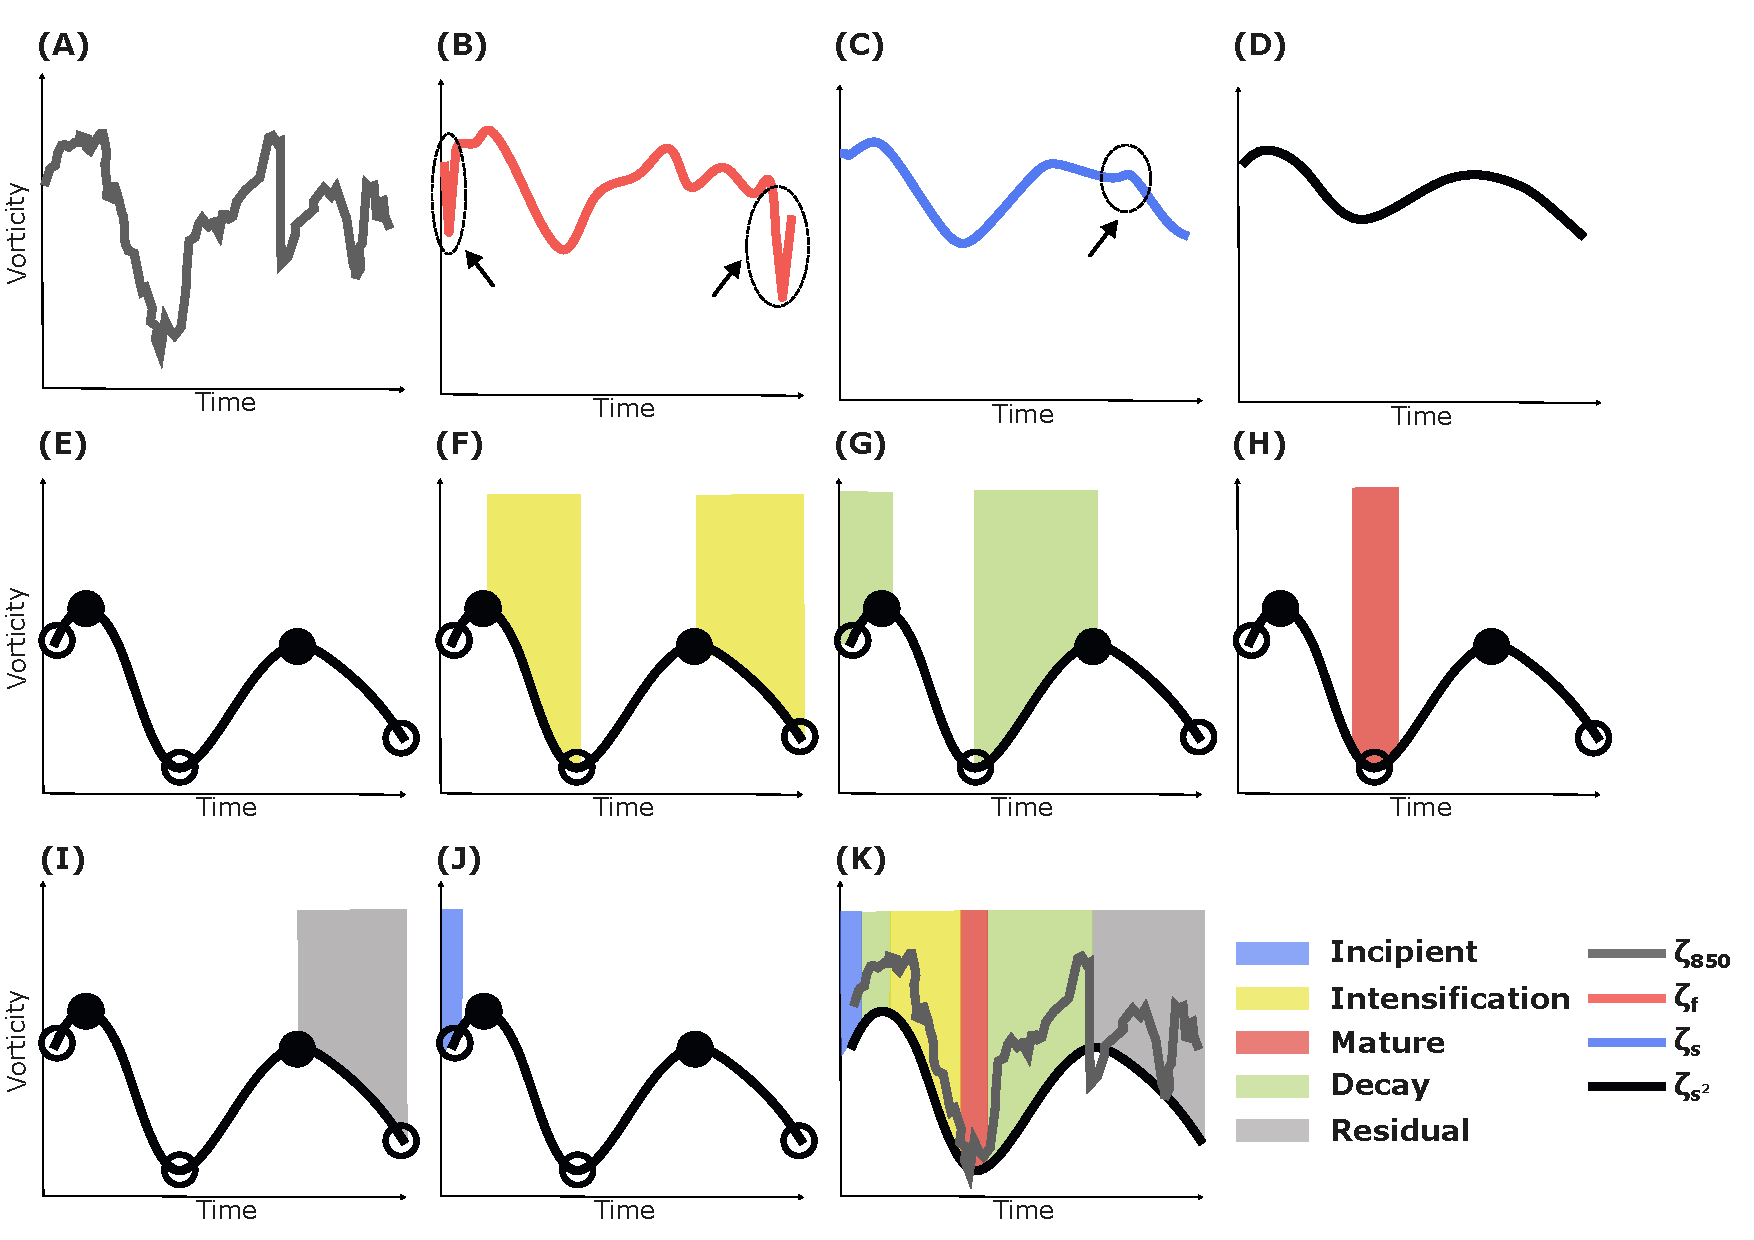
\includegraphics[width=\linewidth]{figs_3/cyclophaser_methodology.pdf}
\caption[Cyclophaser - methodological steps]{Illustrative representation of the methodological steps employed by Cyclophaser in analyzing cyclone lifecycle phases using vorticity series. The detailed steps demonstrate the application of data processing techniques including the Lanczos filter.}
\label{fig:/cyclophaser_methodology}
\end{figure}

The program begins with a preprocessing stage where users have the option to apply the Lanczos filter \citep{duchon1979lanczos} to the vorticity time series (Figure \ref{fig:/cyclophaser_methodology}b). Based on the $sinc$ function, the ideal mathematical representation of a low-pass filter, the Lanczos filter is adapted by windowing the $sinc$ function to a finite range. Cyclophaser utilizes a band-pass filtering technique where weights are calculated using two cutoff frequencies, creating a differential of two $sinc$ functions. This allows the filter to pass a specific frequency range while attenuating frequencies outside this range, permitting customization based on the spatio-temporal resolutions of different reanalysis datasets.

The Lanczos filter's primary use in Cyclophaser is to remove noise unrelated to the development of extratropical cyclones on synoptic scales, including fluctuations due to topography-induced circulations, sea breezes, and spatial and temporal variations in sea surface structures \citep{steele2015modelling, da2017shallow, acevedo2010atmospheric}. High-resolution datasets like ERA5 benefit from this filtering, which effectively reduces noise from structures like frontal systems \citep{hoskins2002new}. However, this filtering step may be omitted for datasets that have been preprocessed by tracking algorithms incorporating spatial filters \citep[e.g.]{murray1991numerical, pinto2005sensitivities, flaounas2014cyclotrack, hoskins2002new}. The Lanczos filter can exhibit issues at discontinuities due to the Gibbs phenomenon and edge effects, leading to spurious oscillations at data series endpoints \footnote{The Lanczos filter, like other finite impulse response filters (FIR), can exhibit issues at discontinuities in the data. These issues arise primarily due to the Gibbs phenomenon and edge effects:

1. \textbf{Gibbs Phenomenon}: The Gibbs phenomenon refers to the overshoot and ringing that occurs near discontinuities when approximating a function with a finite series of basis functions \citep{gibbs1898, hamming1989}. In the context of the Lanczos filter, which utilizes a sinc function, abrupt changes at the edges of the filter window can cause ringing effects at the points of discontinuity in the data.

2. \textbf{Edge Effects}: FIR filters, including the Lanczos filter, can produce artifacts at the boundaries of the data series due to the reliance on data points that may not be available at the edges \citep{oppenheim2009, proakis2006}. Techniques such as zero-padding or reflection are often used to mitigate these effects, but they can still result in artifacts or less accurate filtering near the boundaries.

3. \textbf{Finite Window Length}: The window length of the Lanczos filter determines the number of data points used in the convolution. A finite window length means the filter may not fully capture long-term trends or low-frequency components, especially at the edges, leading to discontinuities or spurious oscillations \citep{smith1997, oppenheim1999discrete}.

4. \textbf{Windowing Effect}: The Lanczos filter uses a windowed $sinc$ function to perform the convolution. While windowing reduces spectral leakage by smoothing the transition at the edges of the filter, it also introduces artifacts, particularly near discontinuities where the transition from one region to another is abrupt \citep{harris1978, mitra2001}.}. To mitigate this, a weaker low-pass Lanczos filter is applied to the initial and final 5\% of the data series, ensuring smoother transitions at the endpoints (Figure \ref{fig:/cyclophaser_methodology}b).

The Lanczos band-pass filter is mathematically formulated as follows:

\begin{equation}
w(n) = 
\begin{cases} 
2 \cdot (\text{cutoff}_\text{high} - \text{cutoff}_\text{low}) & \text{if } n = 0 \\
\left( \text{sinc}(2 \cdot \text{cutoff}_\text{high} \cdot n) - \text{sinc}(2 \cdot \text{cutoff}_\text{low} \cdot n) \right) \cdot \text{sinc}\left(\frac{n}{N}\right) & \text{if } n \neq 0 
\end{cases}
\end{equation}


where $n$ is the index of the weight in the filter window, $w(n)$ is the weight at index $n$, $\text{cutoff}_\text{low}$ and $\text{cutoff}_\text{high}$ are the specified lower and upper cutoff frequencies, respectively, and $N$ is half the length of the filter window. The $sinc$ function is defined as:

\begin{equation}
\text{sinc}(x) = \frac{\sin(\pi x)}{\pi x}
\end{equation}

After the initial filtering, the CycloPhaser program employs the Savitzky-Golay filter \citep{savitzky1964smoothing}, as implemented in SciPy's package \citep{virtanen2020scipy}, to further reduce residual noise. This step is crucial for ensuring that the derivative curves form a sinusoidal pattern, which is essential for precise phase detection (Figure \ref{fig:/cyclophaser_methodology}c). The Savitzky-Golay filter operates by fitting a polynomial of degree \( k \) to a window of \( 2m+1 \) data points centered at each point \( y_i \) in the input signal. The coefficients of this polynomial are determined by minimizing the least squares error between the polynomial and the data points within the window. The smoothed value \( \hat{y_i} \) at the point \( y_i \) is then calculated by evaluating the fitted polynomial at \( x_i \):
\[
\hat{y_i} = \sum_{j=-m}^{m} c_j y_{i+j}
\]
where \( c_j \) are the coefficients derived from the polynomial fit, and \( m \) represents half the window size.

Users have the option to apply this smoothing twice (Figure \ref{fig:/cyclophaser_methodology}d), adjusting the window size \( 2m+1 \) and the polynomial order \( k \) to optimize the balance between noise reduction and data fidelity. This flexibility allows users to fine-tune the filter settings to meet specific requirements based on the spatio-temporal resolutions of various reanalysis datasets.

Subsequently, the first derivative of the relative vorticity is calculated predominantly using second-order finite differences, with central differences applied to interior points and first-order forward or backward differences used for endpoints. This derivative is then subjected to double smoothing with the Savitzky-Golay filter to maintain a sinusoidal pattern in the derivative series. This step is critical for accurately identifying cyclone lifecycle phases, making the dual smoothing process mandatory; omitting this could result in a noisy derivative series, potentially leading to erroneous phase detections, which emphasizes its necessity for reliable analysis.

The first phases to be detected are the intensification and decay stages. The program achieves this by analyzing peaks and valleys in the relative vorticity time series data, as shown in Figure \ref{fig:/cyclophaser_methodology}e. The intensification phase is defined as the period between a peak and the subsequent valley (Figure \ref{fig:/cyclophaser_methodology}f). Conversely, the decay phase is defined as the interval between a valley and the following peak (Figure \ref{fig:/cyclophaser_methodology}g). To ensure that only significant phases are considered, each intensification and decay interval must span at least 7.5\% of the total length of the time series. This threshold helps filter out minor fluctuations that are not indicative of true phase changes. To further refine the accuracy of phase detection, the program checks for multiple blocks of consecutive intensification or decay periods. If the gap between these blocks is smaller than 7.5\% of the total series length, the program merges them into a single period. This merging process is crucial as it prevents the fragmentation of significant phases due to short gaps, thereby providing a more accurate and continuous representation of the intensification and decay stages.

After detecting the intensification and decay stages, the program proceeds to identify the mature stage of the cyclone's life cycle (Figure\ref{fig:/cyclophaser_methodology}h). This stage is determined by analyzing not only the peaks and valleys in the relative vorticity but also the smoothed derivative of vorticity. Between a peak and the subsequent valley (or a valley and the subsequent peak) of the vorticity series, there is always a corresponding valley (or peak) in its derivative. These points indicate periods of maximum intensification or decay of vorticity. The mature stage is defined as the interval between a vorticity valley and an adjusted point calculated based on the derivative of vorticity. Specifically, the mature stage spans from 12.5\% of the time between the preceding derivative valley to 12.5\% of the time to the following derivative peak. To be recognized as a significant mature stage, each interval must span at least 3\% of the total length of the time series. This threshold ensures that only substantial periods are classified as mature stages. Additionally, the program verifies that all mature stages are preceded by an intensification stage and followed by a decay stage. This verification step ensures that the mature phase is accurately identified within the context of the entire cyclone life cycle.

Our methodology introduces the 'residual' stage, which is not directly related to the intrinsic development of extratropical cyclones but rather to peculiarities arising from the tracking algorithms (Figure \ref{fig:/cyclophaser_methodology}i). This stage is exemplified in Figure \ref{residual_study_case}. Panel (a) illustrates the intensification of a cyclonic system near the southernmost part of Argentina. The system reaches maturity, characterized by closed isobars at 850 hPa (Panel b). As the system begins to decay, it displays open isobars and diminished relative vorticity cohesion (Panel c). During its decay, it is influenced by a nearby system that leads to a temporary increase in the magnitude of its central relative vorticity, indicating a temporary re-intensification (Panel d). The tracking algorithm eventually discontinues its tracking, categorizing this late period of intensification as 'residual'—a phase of late intensification that is not associated with the primary development of the cyclone, as depicted in the relative vorticity series (Panel e).

\begin{figure}[h!]
\centering
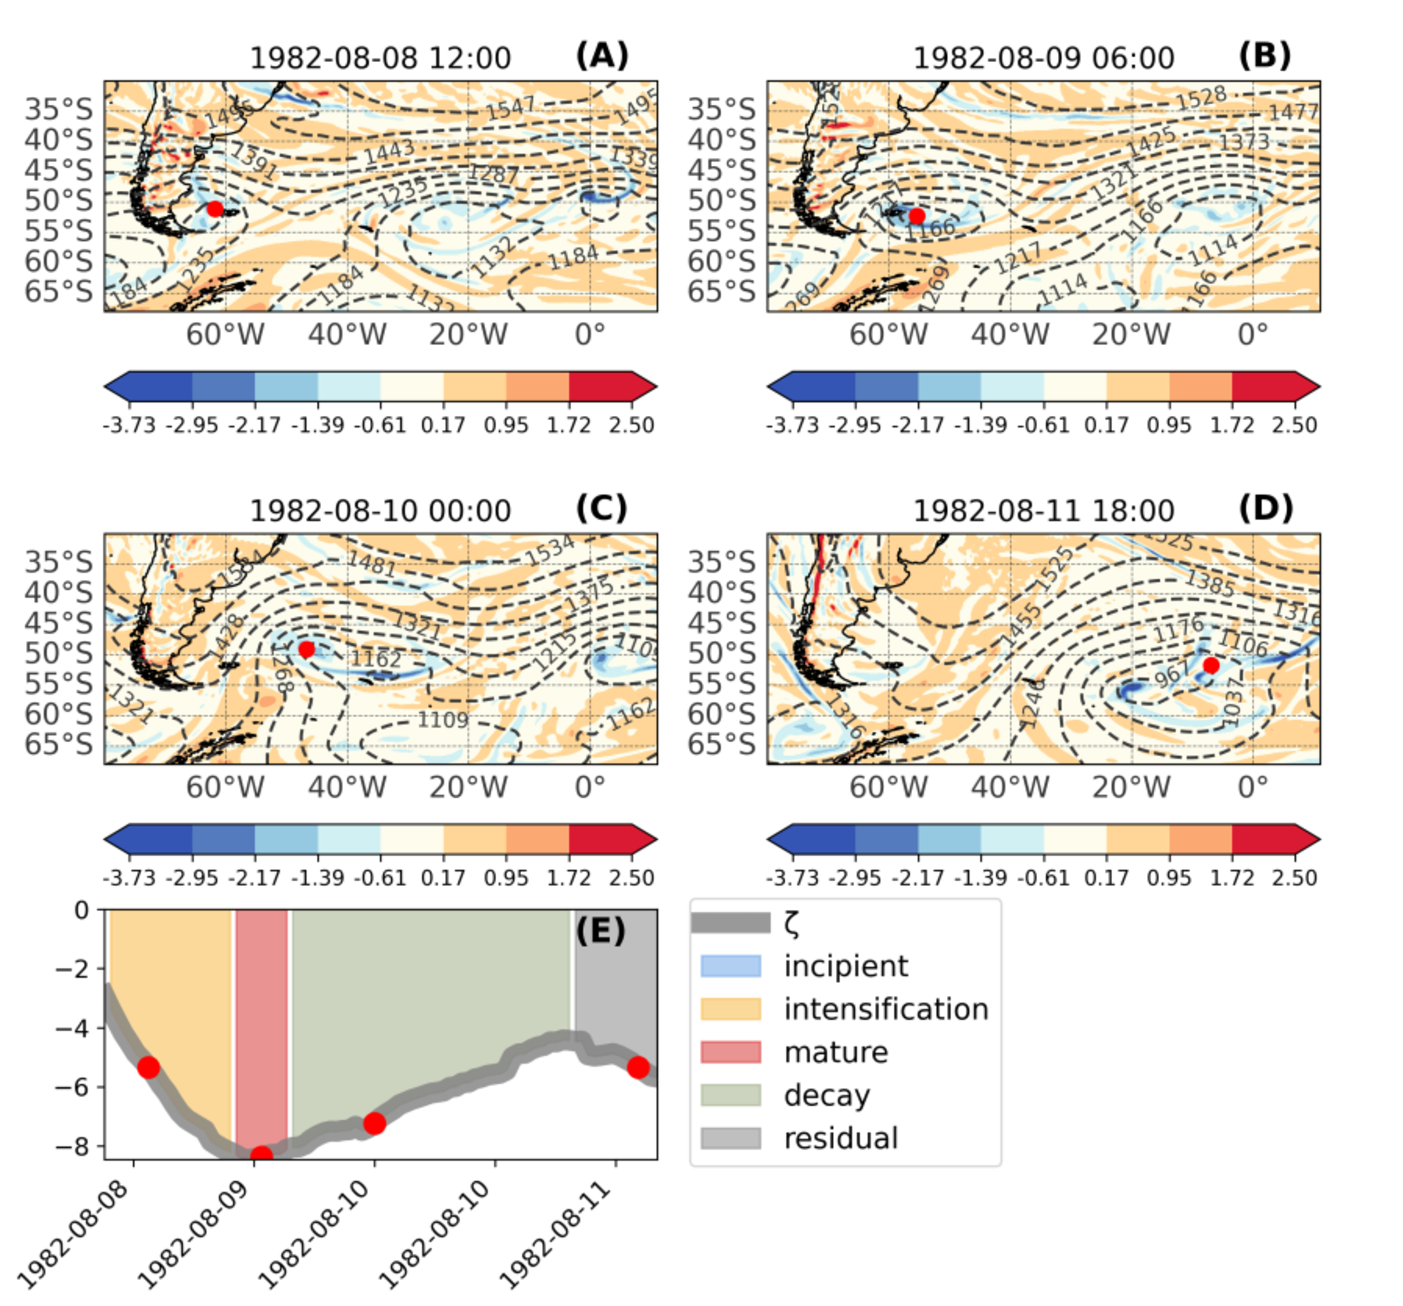
\includegraphics[width=37pc]{figs_3/residual_study_case_edited.pdf}
\caption[Residual stage - study case]{Relative vorticity (shaded) and geopotential heights (contours) at 850 hPa, illustrating distinct stages of a cyclone's lifecycle where a residual stage is present. Panel (A) shows the intensification stage with isobars still open, indicating a strengthening system. Panel (B) depicts the mature stage, characterized by maximum organization and extent. Panel (C) illustrates the decay stage, with open isobars and reduced relative vorticity cohesion. Panel (D) captures the residual phase, where, despite a general trend of weakening, there is a temporary increase in vorticity influenced by external factors, not directly associated with the primary development of the cyclone. The complete lifecycle of the system is depicted in Panel (E), where each red dot on the vorticity series corresponds to the specific moments shown in Panels (A) to (D).}
\label{residual_study_case}
\end{figure}

The CycloPhaser classifies stages as residual by analyzing the previously detected cyclone phases. For phases classified as mature that do not transition to a decay stage, these instances are classified as residual. Similarly, if a full cycle of intensification, maturity, and decay is followed by another intensification that does not lead to a mature phase, it is also classified as residual (Figure \ref{fig:/cyclophaser_methodology}i). This criterion accounts for scenarios where the tracking algorithm may continue to follow a cyclone post-decay, potentially capturing a re-intensification that does not culminate in a mature stage due to tracking limitations.

Following the residual phase classification, a post-processing step is applied to refine cyclone phase identification. This step bridges any gaps that may appear between consecutive periods identified as intensification or decay phases. Specifically, the program scans for discontinuities within consecutive phase blocks and fills any identified gaps with the adjacent phase to ensure smooth and continuous phase transitions. Additionally, this step involves correcting isolated phases—those misclassified phases that last only one time step—by aligning them with the subsequent phase if they occur at the start of the series, or with the preceding phase elsewhere. This adjustment enhances the consistency of phase identification throughout the cyclone lifecycle.

Ironically, the final step of the CycloPhaser program involves identifying the incipient stage, which marks the beginning of cyclone development (Figure \ref{fig:/cyclophaser_methodology}j). Initially, all undefined periods in the time series are labeled as incipient. Subsequently, the program analyzes the sequence of already labeled phases. If the life cycle commences with an intensification phase, the program searches for a vorticity valley preceding the next mature stage. Should such a valley be present, it designates the period from the start of the intensification phase to 40\% of the duration to this valley as incipient. Conversely, if the life cycle starts with a decay phase, the program looks for a subsequent vorticity peak before the next mature stage. Upon identifying such a peak, it marks the time from the start of the decay phase to 40\% of the duration to this peak as incipient.

The specific thresholds for phase detection, including the 7.5\% duration for intensification and decay intervals, the 3\% minimum for the mature stage, and the 12.5\% intervals defining the boundaries of the mature stage, along with 40\% of the series length for the incipient stage, were established through rigorous testing. This testing involved an iterative trial-and-error calibration process where various percentage thresholds were applied to a representative sample of cyclone tracks. The objective was to determine the most accurate parameters for delineating the phases. The chosen percentages proved effective in capturing the true progression of cyclogenesis while filtering out inconsequential fluctuations in vorticity. This meticulous calibration ensures that the CycloPhaser program reliably identifies each phase, providing a consistent and objective methodology for analyzing the life cycle of extratropical cyclones. This process is illustrated in Figures \ref{fig:threshold_intensification} and \ref{fig:threshold_decay}, \ref{fig:threshold_mature}, \ref{fig:threshold_incipient}. For most of these thresholds, and in most cases analyzed, even altering the parameters to 25\% or 150\% of their original values did not result in significant modifications to the identified life cycle, reinforcing the method's reliability.


\begin{figure}[h!]
    \centering
    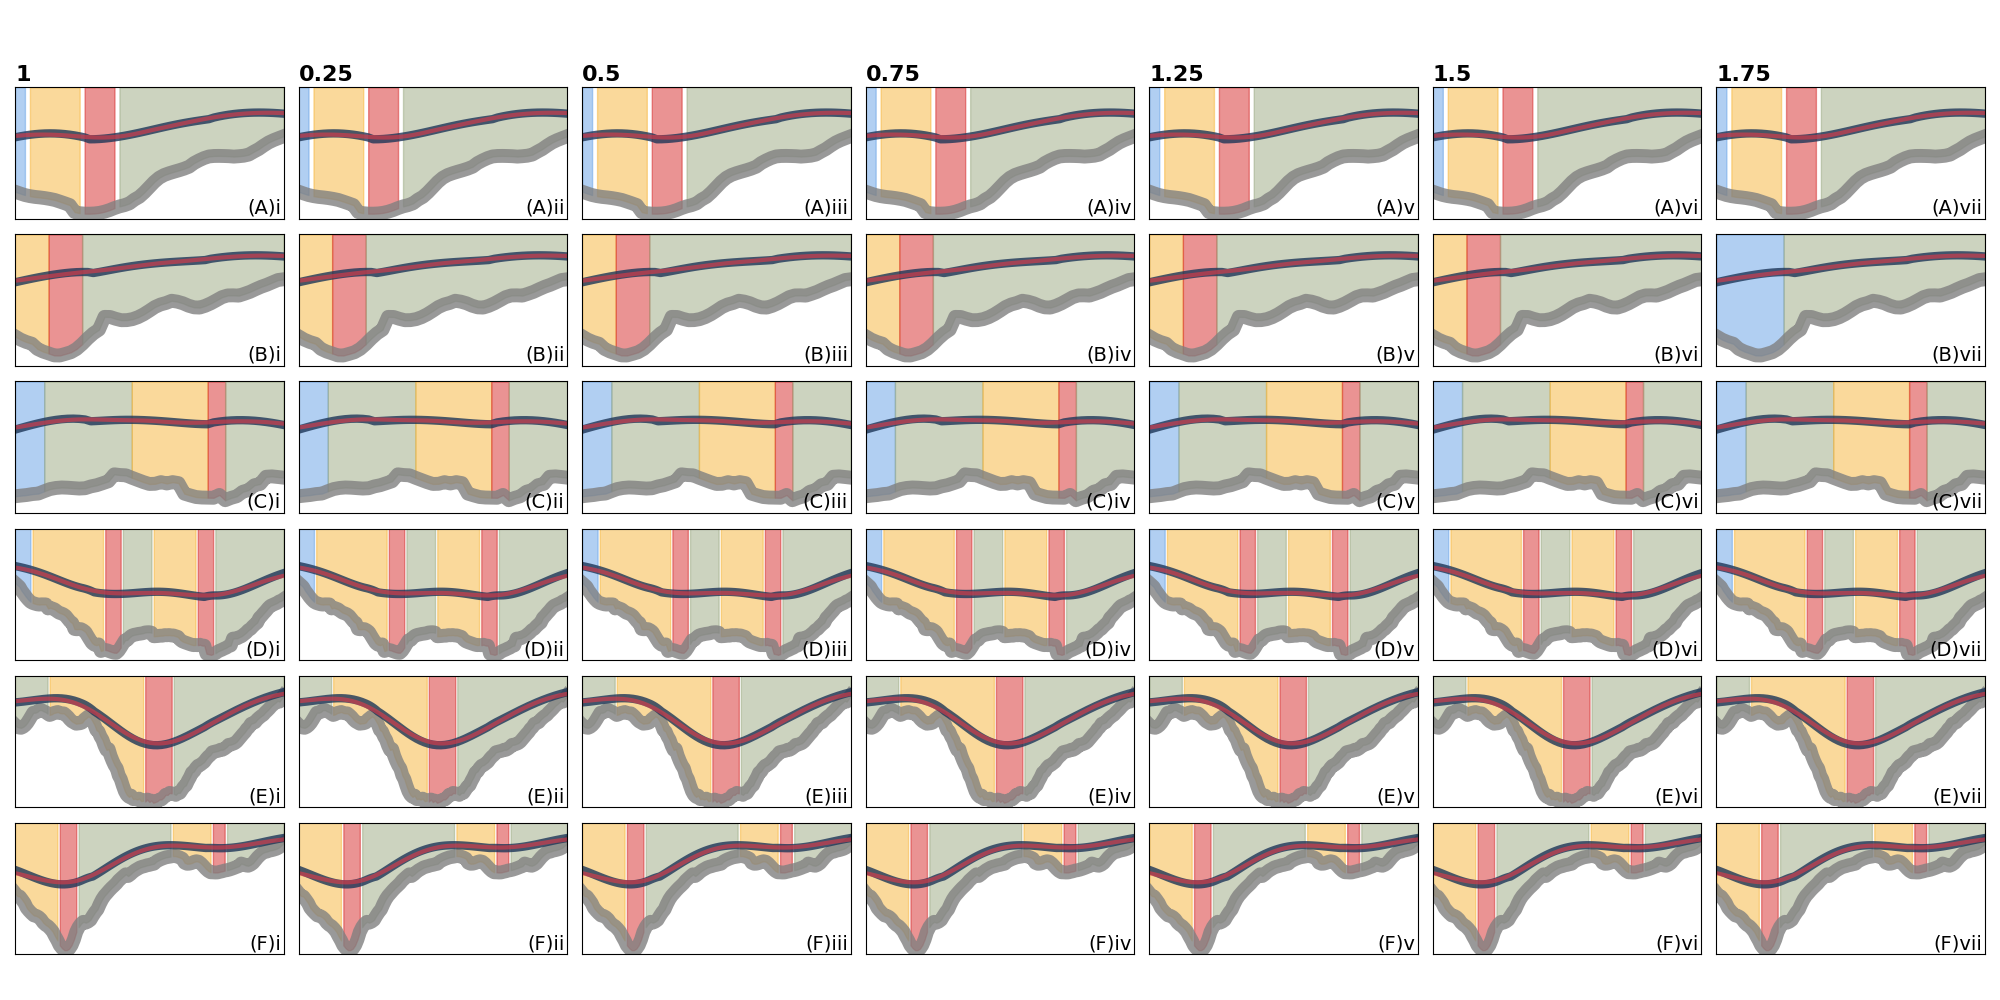
\includegraphics[width=\textwidth]{figs_3/figure_threshold_intensification_length.png}
    \caption[Impact of Varying Threshold Values for Intensification Phase]{Impact of varying threshold values for the minimum length of the intensification phase across the six study cases. The original threshold value is maintained at 7.5\% of the cyclone's total life cycle duration in panel (i). Panels (ii) to (vii) depict variations where the threshold is adjusted from 25\% to 175\% of the original value, illustrating the method's sensitivity to threshold changes. Adapted from \textbf{REFERENCE}.}
    \label{fig:threshold_intensification}
\end{figure}

\begin{figure}[h!]
    \centering
    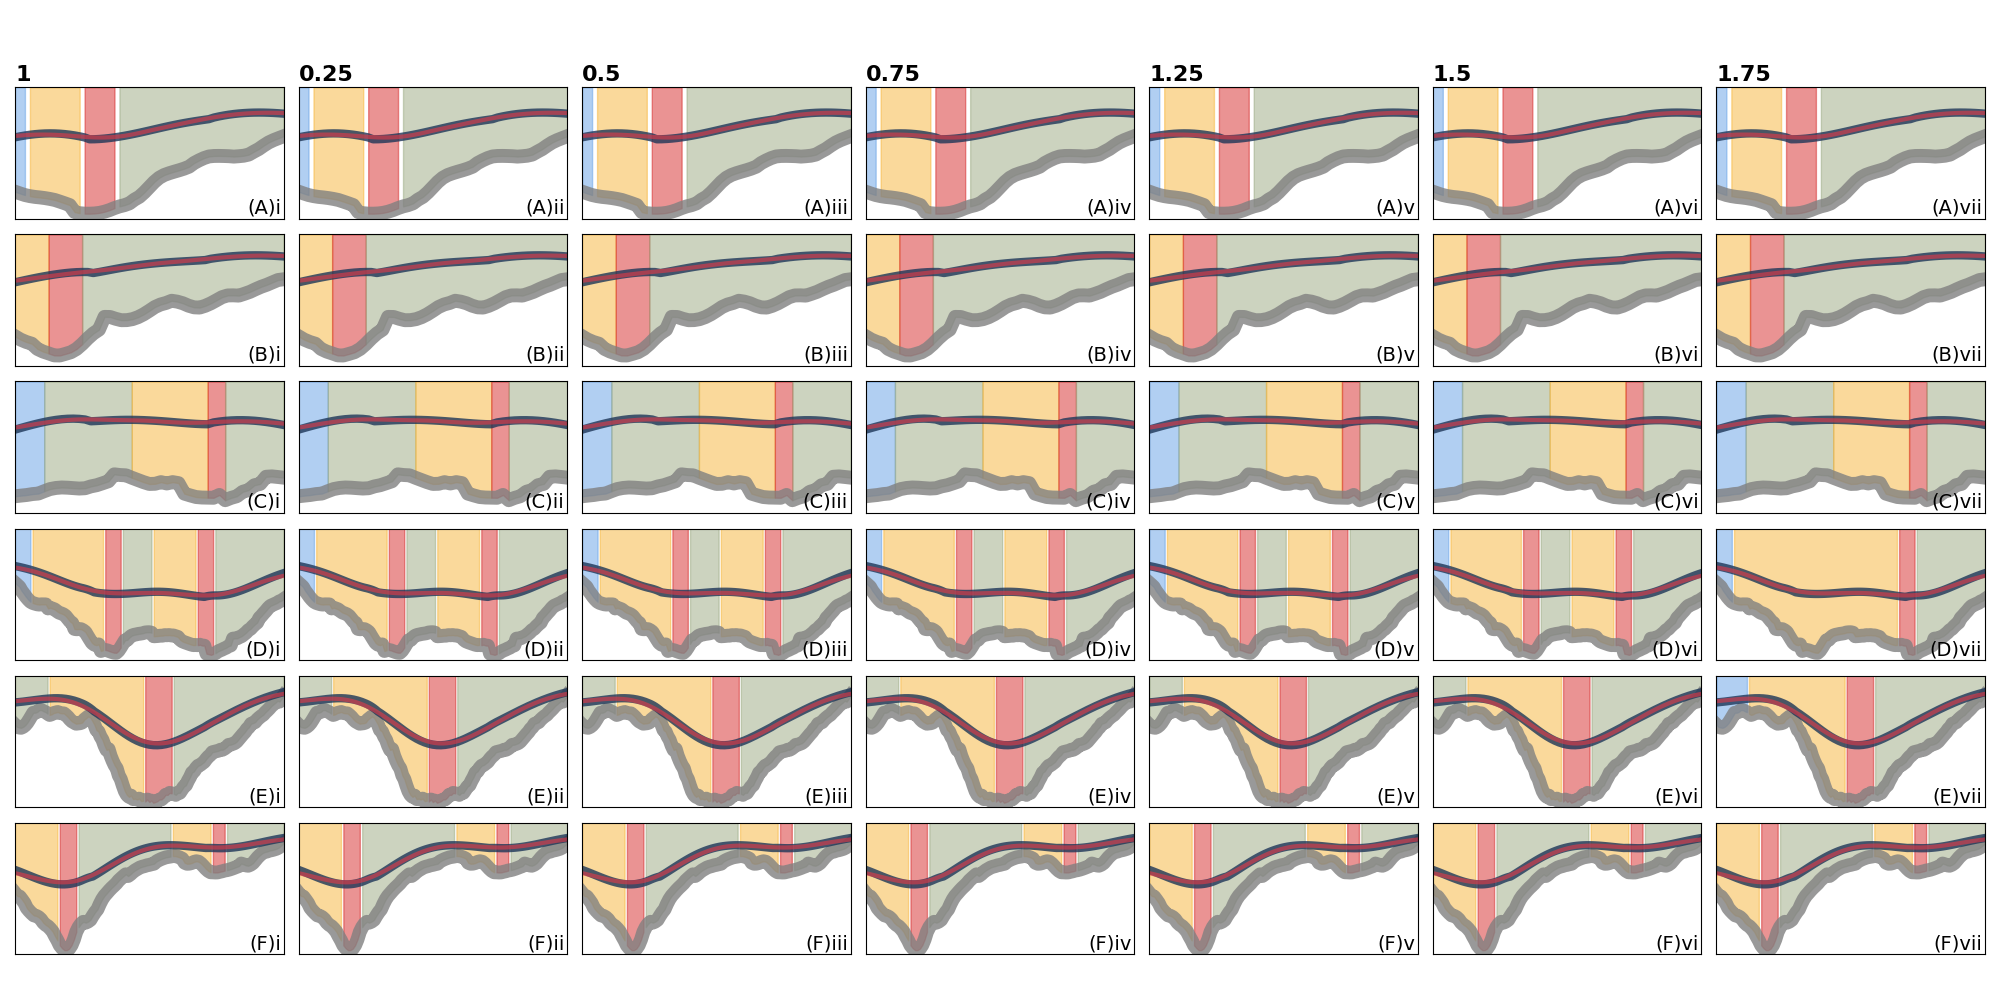
\includegraphics[width=\textwidth]{figs_3/figure_threshold_decay_length.png}
    \caption[Impact of Varying Threshold Values for Decay Phase]{Same as Figure \ref{fig:threshold_intensification}, but for the minimum length of the decay phase. Adapted from \textbf{REFERENCE}.}
    \label{fig:threshold_decay}
\end{figure}

\begin{figure}[h!]
    \centering
    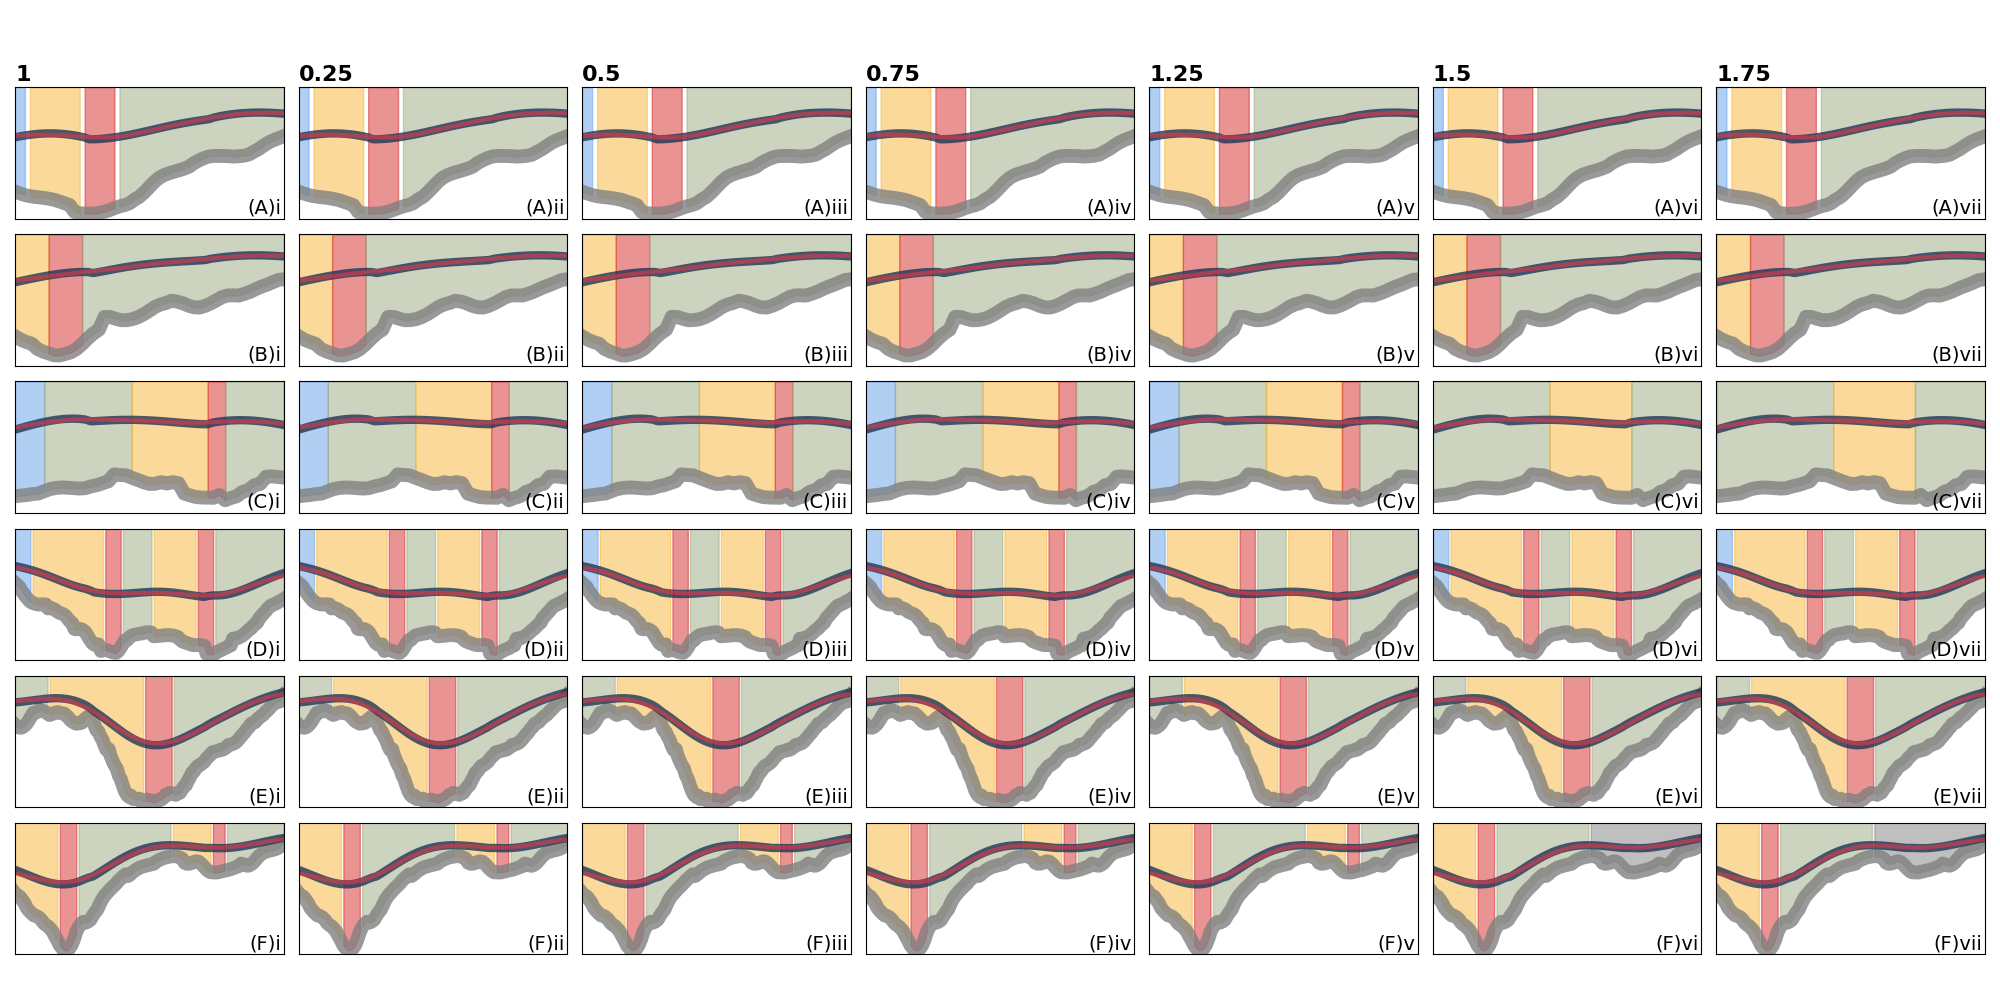
\includegraphics[width=\textwidth]{figs_3/figure_threshold_mature_length.png}
    \caption[Variations in Threshold Values for Mature Phase]{Variations in threshold values for the time intervals between the valley of vorticity and the preceding derivative valley, as well as from the vorticity valley to the subsequent derivative peak, used for determining the mature stage. The original threshold is set at 12.5\%. Subsequent panels adjust this threshold from 25\% to 175\% of the baseline value, evaluating the robustness of phase detection across six study cases. Adapted from \textbf{REFERENCE}.}
    \label{fig:threshold_mature}
\end{figure}

\begin{figure}[h!]
    \centering
    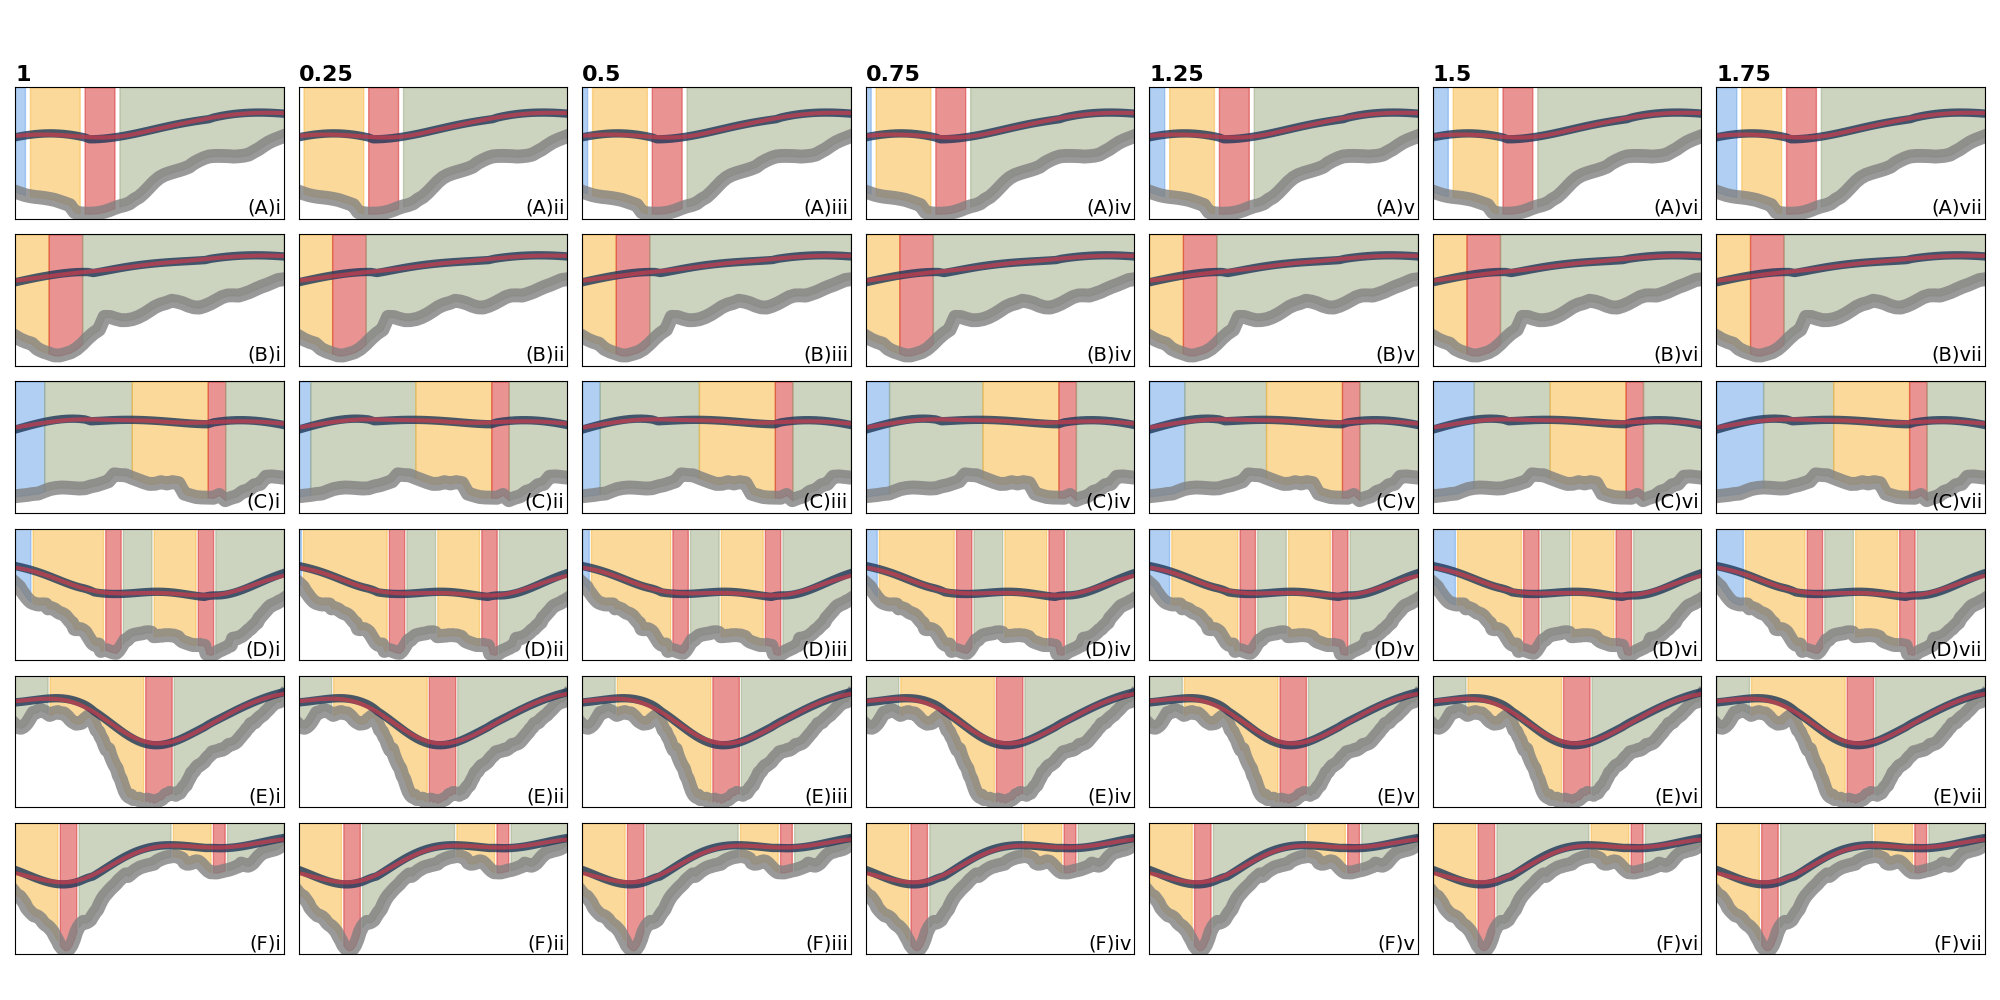
\includegraphics[width=\textwidth]{figs_3/figure_threshold_incipient_length.png}
    \caption[Impact of Varying Threshold Values for Incipient Phase]{Impact of varying the minimum length threshold for the incipient phase of cyclone development. The incipient phase is identified from the beginning of the vorticity series to the next peak or valley in vorticity. The original threshold (shown in panel i) is set based on a percentage of the total vorticity series length. Panels ii to vii display the results when this threshold is modified from 25\% to 175\% of its original value across six study cases. Adapted from \textbf{REFERENCE}.}
    \label{fig:threshold_incipient}
\end{figure}

\subsection{Cyclophaser settings} \label{sec:cyclophaser_settings}

In this study, the default settings of the CycloPhaser were primarily utilized to identify the life cycle phases of cyclones. Since the TRACK algorithm already incorporates spatial filtering on the \(\zeta_{850}\) vorticity fields, application of the Lanczos filter was deemed unnecessary \citep{hodges1994general, hodges1995feature}. Nevertheless, the Savitzky-Golay filter was applied twice to ensure that the \(\zeta_{850}\) series exhibited a smooth sinusoidal profile. The window length of this filter was adjusted specifically for each system's life cycle duration: for systems with a total life cycle spanning 8 days, the window length was set to an odd integer approximately 25\% of the series length. For systems with shorter life cycles, the window length was adjusted to an odd integer approximately 50\% of the series length. In the second smoothing process, for life cycles exceeding 8 days, the window length was set to an odd integer close to 50\% of the series length; however, for shorter cycles, it was kept consistent with the initial smoothing step.


\section{Cálculo do ciclo energético}\label{metodos_calculo_lec}

\begin{itemize}
    \item Programa de calculo do LEC (Github) e procedimentos adotados para os cálculos
\end{itemize}

\section{Determinação dos padrões energéticos}

\begin{itemize}
    \item Padronização da duração dos sistemas através do ciclo de vida
    \begin{itemize}
        \item Cyclophaser
    \end{itemize}
    \item Diagrama de fase (Lorenz Phase Space)
    \item Cálculo da PCA dos termos
    \item Método K-means

\end{itemize}

\section{Descrição do MPAS-A}

\begin{itemize}
    \item Visão geral do modelo
    \item  Descrição do núcleo dinâmico e discretizações numéricas
    \item Malha adotada e estrutura de grade (horizontal e vertical)
    \item Opções disponíveis de parametrizações físicas
\end{itemize}

\section{Desenho experimental das simulações}

\subsection{Testes de sensibilidade: Furacão Catarina}
\begin{itemize}
\item Desenho dos experimentos
\begin{itemize}
    \item Combinações de parametrizações físicas e de cumulus
    \item Duração de cada set de experimentos (3 períodos de 48h cada)
\end{itemize}
\item Inicialização do modelo
\item Estrutura de grade adotada (horizontal e vertical)
\end{itemize}

\subsection{Experimentos com SST}
\begin{itemize}
    \item Casos escolhidos
    \item Pertubações adotadas
\end{itemize}